\documentclass{beamer}

\mode<presentation>
{
  \usetheme[hideothersubsections]{MorrisStyle}
  \setbeamercovered{transparent}
}

\usepackage[english]{babel}
\usepackage[latin1]{inputenc}
\usepackage{times}
\usepackage[T1]{fontenc} 
\usepackage{amsmath}

\newcommand{\linespace}{\vskip 0.25cm}

\definecolor{MyForestGreen}{rgb}{0,0.7,0} 
\newcommand{\tableemph}[1]{{#1}}
\newcommand{\tablewin}[1]{\tableemph{#1}}
\newcommand{\tablemid}[1]{\tableemph{#1}}
\newcommand{\tablelose}[1]{\tableemph{#1}}

\definecolor{MyLightGray}{rgb}{0.6,0.6,0.6}
\newcommand{\tabletie}[1]{\color{MyLightGray} {#1}}

% The text in square brackets is the short version of your title and will be used in the
% header/footer depending on your theme.
\title[Energy Optimization Techniques]{Modern Energy Optimization Techniques for a Green Cloud}

% Sub-titles are optional - uncomment and edit the next line if you want one.
% \subtitle{Why does sub-tree crossover work?} 

% The text in square brackets is the short version of your name(s) and will be used in the
% header/footer depending on your theme.
\author[Donatucci]{David Donatucci}

% The text in square brackets is the short version of your institution and will be used in the
% header/footer depending on your theme.
\institute[UMM]
{
  Division of Science and Mathematics \\
  University of Minnesota, Morris \\
  Morris, Minnesota, USA
}

% The text in square brackets is the short version of the date if you need that.
\date[December '14, Senior Seminar] % (optional)
{December 6th 2014 \\ Senior Seminar Conference, Morris, MN}

% Delete this, if you do not want the table of contents to pop up at
% the beginning of each subsection:
\AtBeginSection[]
{
  \begin{frame}<beamer>
    \frametitle{Outline}
    \tableofcontents[currentsection, hideothersubsections]
  \end{frame}
}

\begin{document}

\begin{frame}
  \titlepage
\end{frame}

% For a 20-25 minute senior seminar talk you probably want something like:
% - Two or three major sections (other than the summary).
% - At *most* three subsections per section.
% - Talk about 30s to 2min per frame. So there should probably be between
%   15 and 30 frames, all told.

\section*{Overview}

\subsection*{The Big Picture}

\begin{frame}
  \frametitle{The Big Picture}
  

\begin{columns}
\begin{column}{0.55\textwidth}
  \begin{itemize}
	\item Data centers account for a significant fraction of all electricity used in the world.
	\item Large demand for cloud computing means providers must find ways to reduce energy.
	\item Implementing green algorithms may be used to improve data center efficiency.  
  \end{itemize}
\end{column}
\begin{column}{0.45\textwidth}

\includegraphics[width=.95\textwidth]{GreenCloud.jpg} \\
\tiny{Green Cloud, http://coaster.tempdomainname.com}
\end{column}
\end{columns}
  
\end{frame}

\subsection*{Outline}

\begin{frame}
  \frametitle{Outline}
  \tableofcontents[hideallsubsections]
\end{frame}

\section[Cloud Computing]{Cloud Computing Basics}

\subsection{Cloud Computing}

\begin{frame}
  \frametitle{Cloud Computing}
 \begin{columns}
	\begin{column}{0.55\textwidth}
 		\large{\textbf{What is the Cloud?}}
 		\begin{itemize}
 			\item Application services
 				\begin{itemize}
 					\item Shared calendar
 				\end{itemize}
 			\item Hardware and software systems
 			\linebreak 
 			\item Data centers 
 				\begin{itemize}
 					\item Remote servers
 				\end{itemize}
 			\item Centralization of data storage and processing
 		\end{itemize}
	\end{column}
\begin{column}{0.45\textwidth}
	
\includegraphics[width=1.0\textwidth]{GreenQuestionMark.jpg} \\
	\tiny{
		\begin{flushright}
			http://blog.neoxia.com/
		\end{flushright}
	}
	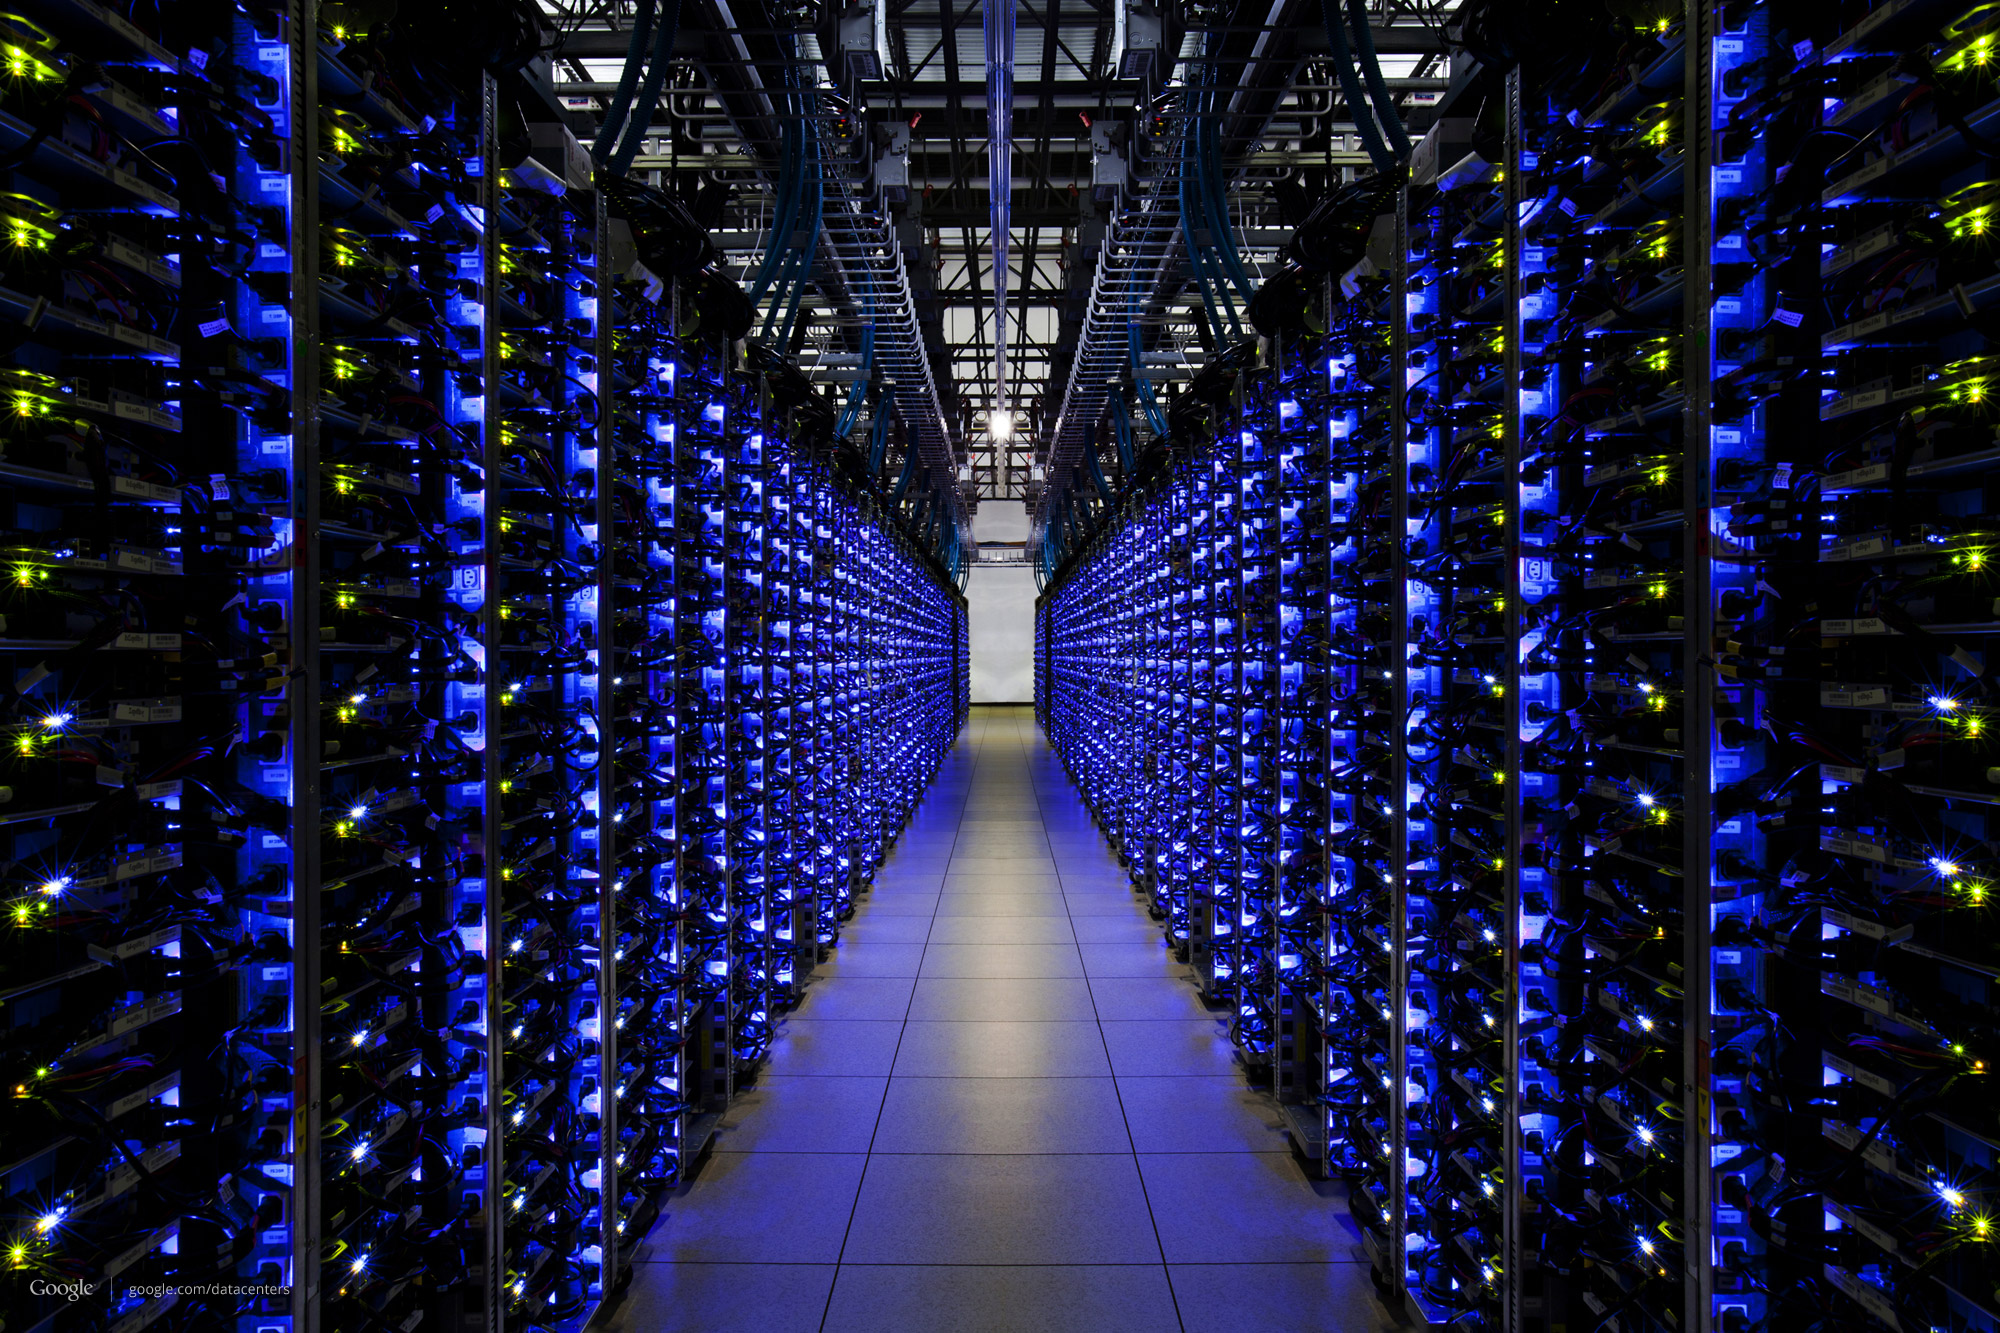
\includegraphics[width=1.0\textwidth]{Servers.jpg} \\
	\tiny{
		\begin{flushright}
			http://www.coldcreeksolutions.com/
		\end{flushright}
	}
\end{column}
\end{columns}
\end{frame}

\begin{frame}
  \frametitle{Cloud Computing Terminology}
	\emph{Requests}:	A user tries to access a particular service. 
	\linebreak
	\linebreak
	\emph{Workload}: Number of requests for all services at a given time.
	\linebreak
	\linebreak
	\emph{Workload capacity}: Total number of requests a data center can handle at any given time.
	\linebreak
	\linebreak
	\emph{Service capacity}, $\Omega$: Total number of services a single server can handle at a given time.
	\linebreak
	\linebreak
	A cloud is in \emph{overload} if number of requests is greater than the service capacity
	\linebreak
	\linebreak
	A cloud is in \emph{underload} if number of requests is less than the service capacity.
	

\end{frame}

\begin{frame}
  \frametitle{Cloud Computing and Energy}
 Cloud Computing has been growing rapidly.  
 \linebreak
 \linebreak
 $\implies$ additional and larger data centers.
 \linebreak
 \linebreak
 $\implies$ more power consumed.
 \begin{description}
 	\item[2000] Data centers used ~70 Terawatts hours worldwide (.5\%)
 	\item[2010] Data centers used ~280 Terawatts hours worldwide (1.5\%)
 \end{description}  

\end{frame}

\subsection[Macro vs Micro]{Macro vs Micro Algorithms}

\begin{frame}
  \frametitle{Macro vs Micro Algorithms}
 	Two Types of Energy Optimization Techniques
 		\begin{enumerate}
 			\item Macro Algorithms:
 				\begin{itemize}
 					\item Geographic location
 					\item Climate
 					\linebreak
 				\end{itemize}
 			\item Micro Algorithms:
 				\begin{itemize}
 					\item Resource Allocation
 				\end{itemize}
 		\end{enumerate}

\end{frame}

\section[Green Monster]{Green Monster (Macro)}

\begin{frame}
	\frametitle{Green Monster}
\begin{columns}
\begin{column}{0.55\textwidth}
	\begin{itemize}
	\item Framework for multiple data centers.
	\linebreak
	\item Attempts to take advantage of diverse climates and renewable resources.
	\linebreak
	\item EMOA
	\end{itemize}

\end{column}
	\begin{column}{0.45\textwidth}
	\includegraphics[width=1.0\textwidth]{GreenMonster.jpg} \\
\end{column}
\end{columns}
\end{frame}
\subsection{EMOA}
\begin{frame}
  \frametitle{Evolutionary Multi-Objective Optimization Algorithms}
\begin{columns}
\begin{column}{0.65\textwidth}
  \begin{itemize}
 		\item Evolutionary Multi-Objective Optimization Algorithm (EMOA)
 		\begin{itemize}
 			\item Based upon biological principles.
 			\item Individuals form a population.
 		\end{itemize}
	\item Multiple Optimizations
 		\begin{enumerate}
			\item Renewable Energy (RE)
			\item Cooling Energy (CE)
			\item User-to-Service Distance (USD)
		\end{enumerate}
	\item Three Steps in EMOA: 
		\begin{enumerate}
			\item Initialization
			\item Evolution
			\item Termination
		\end{enumerate}
  \end{itemize}
\end{column}
\begin{column}{0.35\textwidth}
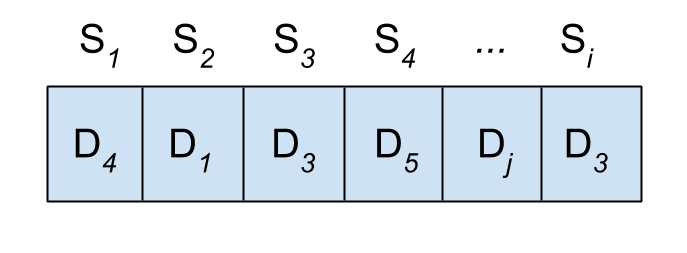
\includegraphics[width=.95\textwidth]{Individual.png} \\
\tiny{Example of an Individual. $S_i$ indicates a service, $D_j$ indicates a data center.}
\linebreak
\linebreak
\linebreak

\end{column}
\end{columns}


\end{frame}
 	
\subsection{EMOA Steps}
\begin{frame}
\frametitle{EMOA Initialization}
  \begin{itemize}
	\item Individuals length is equivalent to number of services.
	\linebreak
	\linebreak
	\item Each service is assigned to a random data center. 
	\linebreak
	\linebreak
	\item Capacity aware randomization.
	\linebreak
	\linebreak
	\item Creates 100 individuals in the first generation.
  \end{itemize}
\end{frame}

\begin{frame}
	\frametitle{EMOA Evolution}
	Binary Tournament
	\begin{itemize}
		\item Best parent selection of two randomly selected individuals: \emph{i}, \emph{j}
		\item Constrained-dominance 
		\linebreak
		\linebreak
		An individual is constrained-dominant if:
			\begin{itemize}
				\item both \emph{i}, \emph{j} are have service violations, the individual with minimum of number of service violations
				\item \emph{i} has service violations and \emph{j} doesn't, \emph{j} is constrained-dominant
				\item both \emph{i}, \emph{j} don't have service violations, individual with greater or equal objective values in all objectives
			\end{itemize}

	\end{itemize}
\end{frame}

\begin{frame}
\frametitle{EMOA Evolution continued and Termination}
  \begin{itemize}
	\item Transformations
		\begin{itemize}
		\item Crossover (90\%)
		\item Mutation (10\%)
		\item Local Search (10\%)
		\item Elitism (N+N)
		\end{itemize}
	\item Termination: Transformations occur over 100 Generations.
  \end{itemize}
\includegraphics[width=.5\textwidth]{Crossover.png}
\includegraphics[width=.5\textwidth]{Mutation.png}
\end{frame}

\subsection[Simulations]{Green Monster Simulations}

\begin{frame}
\frametitle{Simulations}
	Simulated in nine different countries in Europe. \linebreak
	\linebreak
	Temperatures from 2010 real-world data.
	\linebreak
	\linebreak
	Renewable energy of each country from real-world 2007-2009 data. 
	\linebreak
	\linebreak
	Each data center had
		\begin{itemize}
			\item 8-200 servers
			\item 16-400 services
			\item 3 types of service voice, data, video
	
		\end{itemize}
		EMOA run bi-weekly for 12 simulated months.
\end{frame}

\section[GRMP-Q]{Gossip-based Resource Allocation}

\begin{frame}
	\frametitle{Gossip-based Resource Allocation (GRMP-Q)}
		\includegraphics[width=.5\textwidth]{Cloud.jpg}

	\begin{itemize}
		\item Middle-ware for a single data center.
		\item Attempts to reduce number of running servers using gossip protocol.
		\item Assume that all servers have identical specifications.
		\item Two Objectives:
			\begin{enumerate}
				\item Satisfy user demand.
				\item Minimize power consumption.
			\end{enumerate}
	\end{itemize}
\end{frame}

\begin{frame}
	\frametitle{GRMP-Q Set-up}
	
	\begin{itemize}
		\item \emph{N} servers
		\item Service $S_i$
		\item Demand of single server  \emph{n} for a service $S_i$, $\omega$
		\begin{equation}
\omega_{(S_{i},n)} = \alpha_{(S_{i},n)} \omega_{S_i} \text{\emph{~such that~}} \alpha_{(S_{i},n)} \geq 0,~ \sum_{n=1}^{N} \alpha_{(S_{i},n)} = 1 \label{eq:1}
\end{equation}
	\item $\alpha$ is portion of demand on server \emph{n}
	\item Configuration matrix is all the  $\alpha 's$ in matrix form.
	\item Configuration matrix updated on load changes
	\end{itemize}
\end{frame}

\begin{frame}
	\frametitle{Gossip Protocol}
	\begin{itemize}
		\item To Transfer Services to another server:
			\begin{enumerate}
				\item Initialization: starts gossip-protocol with current configuration matrix.
				\item Peer Selection: 
					\begin{itemize}
						\item Selection of \emph{j} from $N_n$, servers with similar services to \emph{n}\\
					$p = \frac{|N_{n}|}{1+|N_{n}|}$
						
						\item Selection from different services 1-p
					\end{itemize}
					
				\item Migration Calculation:
				\begin{itemize}
				\item Calculate relative demand of \emph{j} and \emph{n}, $y_n$ where \\
				$y_n = \sum_{i=1}^M \frac{\omega_{(S_i,n)}}{\Omega} \textit{~where M is the total num of services}$
				\item if $y_n+y_j \geq 2$, assumes overloaded cloud.
				\item if $y_n+y_j < 2$, assumes underloaded cloud.
				
				\end{itemize}
				\item Migration:
				\begin{itemize}
				\item Underload: Packs server with highest relative demand so that equals $\Omega$.
				\item Overload: Pack excess to a new service in which $\alpha = 0$ in the configuration matrix. 
				
				\end{itemize}
			\end{enumerate} 
	\end{itemize}
\end{frame}


\section[Results]{Results}
\subsection{Green Monster}
\begin{frame}
	\frametitle{Green Monster Results}
	Two Benchmark algorithms: Static and Random
	\begin{itemize}
		\item Increased about 33.3\% in renewable energy consumption.
	\item Reduced cooling energy consumption by 3.2\%
	\item Reduced USD to 23.4\%	
	\end{itemize}

	
	\begin{table}[tb]
\begin{center}
\begin{tabular}{|l|l|l|l|}
    \hline
    \multicolumn{4}{|c|}{\textbf{Daily Averaged Objective Values for Green Monster}} \\
    \hline
    & Renewable &  Cooling & User-to-Service \\
    & Energy & Energy & Distance \\
    \hline
    Static & 324.5 & 949.58 & 0 \\
    Random & 327.3 & 947.34 & 487378\\
   	Green Monster & 438.5 & 919.02 & 373172\\
    \hline
\end{tabular}
\caption{Daily averaged objective values for static placement, random placement, and Green Monster. RE and CE are in MWh. USD is presumed to be in meters. }
\label{tab:GMV}
\end{center}
\end{table}
	
\end{frame}
\subsection{GRMP-Q}
\begin{frame}
	\frametitle{GRMP-Q Results}
	Simulation with 10,000 servers.
	\begin{itemize}
		\item Reduced energy consumption by 80\% at 10\% CPU demand.
		\item No reduction in overload.
		\item Scalable to 160,000 servers.
	\end{itemize}
	
	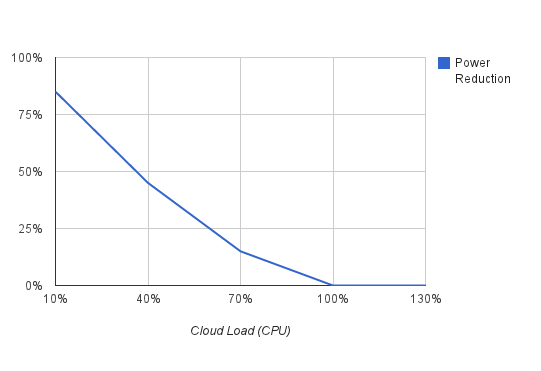
\includegraphics[width=.7\textwidth]{image.png}
	
\end{frame}
\section{Conclusions}
\begin{frame}
	\frametitle{Conclusions}
	\begin{itemize}
		\item Implementing energy optimization algorithms important for a green cloud. 
		\linebreak
		\item Simulated results, need to obtain experimental results.
		\linebreak
		\item Since algorithms are distinct could be combined for greater savings.
	\end{itemize}
\end{frame}
\section*{References}

\begin{frame} 
\frametitle{References}
\nocite{*}
\bibliographystyle{acm}
{\tiny \bibliography{annotated_bibliography}}
\end{frame} 

\end{document}